% 宏包和设置
% zihao 命令,小N号用 -N,大N号用 +N
\documentclass[zihao=-4,openany,fancyhdr,UTF8]{ctexbook}
\usepackage{amsmath,amssymb,amsthm} % 美国数学协会
\usepackage{physics} % 物理
\usepackage{graphicx} % 图片
\usepackage{xcolor} % 颜色控制
\usepackage[framemethod=TikZ]{mdframed} % 框
\usepackage[final]{pdfpages} % 页面插入 pdf
\usepackage{listings} % 代码排版
\usepackage{bm} % 用于矢量的粗体
\usepackage{etoolbox}
\setboolean{@twoside}{false} % 封面只占一面
\usepackage{enumitem}  % \begin{enumerate}[resume] 可以接着之前的编号
\usepackage{siunitx} % 单位
\usepackage{mathrsfs} % 使用 \mathscr 花体字母
\usepackage{newtxtext}
\allowdisplaybreaks
\usepackage[sectionbib]{natbib}
\setcitestyle{numbers,square}
% 数学格式

%表示角度的圆圈直接用° (搜狗打du即可)
\newcommand{\I}{\mathrm{i}} %虚数单位正体
\newcommand{\E}{\mathrm{e}} %自然对数底整体
\newcommand{\bvec}[1]{\boldsymbol{\mathbf{#1}}} %矢量用正体加粗字母, 大写也可以(电场) %只用 mathbf 对希腊字母没用
\newcommand{\mat}[1]{\boldsymbol{\mathbf{#1}}}   %矩阵用正体加粗字母, 小写也可以(泡利矩阵)
\newcommand{\ten}[1]{\boldsymbol{\mathbf{#1}}} % 张量与矩阵相同
\newcommand{\Nabla}{\bvec\nabla} % 粗体 nabla
%\renewcommand{\laplacian}{\bvec{\nabla}^2} % 粗体拉普拉斯算符, 覆盖 physics 宏包
\renewcommand{\Tr}{^{\textup{T}}} %矩阵转置 % 覆盖 physics 宏包的 Trace
\newcommand{\uvec}[1]{\hat{\boldsymbol{\mathbf{#1}}}} %单位矢量为黑体加 hat
\renewcommand{\pmat}[1]{\begin{pmatrix}#1\end{pmatrix}} % 矩阵圆括号, 覆盖 physics 宏包 (pauli matrix)
\newcommand{\ali}[1]{\begin{aligned}#1\end{aligned}}
\newcommand{\leftgroup}[1]{\left\{\begin{aligned}#1\end{aligned}\right.}
\newcommand{\vmat}[1]{\begin{vmatrix}#1\end{vmatrix}} % 行列式
\newcommand{\bmat}[1]{\begin{bmatrix}#1\end{bmatrix}} % 方括号矩阵
\newcommand{\Bmat}[1]{\left\{\begin{matrix}#1\end{matrix}\right\}} % 花括号矩阵
\newcommand{\Cj}{^*} % 复共轭
\newcommand{\dfracH}{\rule[-0.5cm]{0pt}{1.3cm}} % 全尺寸分数 dfrac 在表格中的高度
\newcommand{\Her}{^\dagger} %厄米共轭
\newcommand{\Q}[1]{\hat{#1}} % 量子力学算符
\newcommand{\Qv}[1]{\uvec #1} % 量子力学矢量算符
\newcommand{\opn}{\operatorname} % 算符与函数的简写
\newcommand{\sinc}{\operatorname{sinc}} % sinc 函数
\newcommand{\erfi}{\operatorname{erfi}} % erfi 函数
\newcommand{\Arctan}{\operatorname{Arctan}} % Arctan 函数
\newcommand{\Si}[1]{\ \si{#1}} % 国际单位
\DeclareMathOperator*{\sumint}{% 求和加积分符号
\mathchoice%
  {\ooalign{$\displaystyle\sum$\cr\hidewidth$\displaystyle\int$\hidewidth\cr}}
  {\ooalign{\raisebox{.14\height}{\scalebox{.7}{$\textstyle\sum$}}\cr\hidewidth$\textstyle\int$\hidewidth\cr}}
  {\ooalign{\raisebox{.2\height}{\scalebox{.6}{$\scriptstyle\sum$}}\cr$\scriptstyle\int$\cr}}
  {\ooalign{\raisebox{.2\height}{\scalebox{.6}{$\scriptstyle\sum$}}\cr$\scriptstyle\int$\cr}}
}

\newcommand{\bibentry}[1]{ \\ \vspace{-0.34cm}\input{./bibliographies/#1}} % 文献词条

% 设置 Matlab 格式,用于MatlabStyle.tex
\usepackage{color} %red, green, blue, yellow, cyan, magenta, black, white
\definecolor{mygreen}{RGB}{28,172,0}
\definecolor{mylilas}{RGB}{170,55,241}
\definecolor{string}{RGB}{160,32,240}
\definecolor{comment}{RGB}{34,139,34}
\definecolor{warning}{RGB}{255,100,0}
\definecolor{error}{RGB}{230,0,0}
\definecolor{background}{RGB}{252,252,220}

% 其他
\newcommand{\entry}[2]{\section{#1}\phantomsection\label{#2}\input{./contents/#2}}% 主程序中使用,从 contents 文件夹加入词条
\newcommand{\pentry}[1]{\begin{mdframed}\textbf{预备知识\ } #1 \end{mdframed}\vspace{-0.3cm}\par}%预备知识的格式
\newcommand{\rentry}[1]{\begin{mdframed}\textbf{拓展阅读\ } #1 \end{mdframed}\vspace{-0.3cm}\par}%拓展阅读的格式
\newcommand{\eentry}[1]{\begin{mdframed}\textbf{应用举例\ } #1 \end{mdframed}\vspace{-0.3cm}\par}%应用举例的格式

% 淘宝模板其他设置
\mdfsetup{%
frametitlealignment=\noindent\raggedright,
middlelinecolor=gray,
middlelinewidth=.3pt,
backgroundcolor=white,
roundcorner=6pt}
%-------------------------------------------------------------------------------
% Colors adapted from Material Design
%-------------------------------------------------------------------------------

% Red
\definecolor{red-50}{RGB}{255,235,238}
\definecolor{red-100}{RGB}{255,205,210}
\definecolor{red-200}{RGB}{239,154,154}
\definecolor{red-300}{RGB}{229,115,115}
\definecolor{red-400}{RGB}{239,83,80}
\definecolor{red-500}{RGB}{244,67,54}
\definecolor{red-600}{RGB}{229,57,53}
\definecolor{red-700}{RGB}{211,47,47}
\definecolor{red-800}{RGB}{198,40,40}
\definecolor{red-900}{RGB}{183,28,28}
\definecolor{red-A100}{RGB}{255,138,128}
\definecolor{red-A200}{RGB}{255,82,82}
\definecolor{red-A400}{RGB}{255,23,68}
\definecolor{red-A700}{RGB}{213,0,0}

% Pink
\definecolor{pink-50}{RGB}{252,228,236}
\definecolor{pink-100}{RGB}{248,187,208}
\definecolor{pink-200}{RGB}{244,143,177}
\definecolor{pink-300}{RGB}{240,98,146}
\definecolor{pink-400}{RGB}{236,64,122}
\definecolor{pink-500}{RGB}{233,30,99}
\definecolor{pink-600}{RGB}{216,27,96}
\definecolor{pink-700}{RGB}{194,24,91}
\definecolor{pink-800}{RGB}{173,20,87}
\definecolor{pink-900}{RGB}{136,14,79}
\definecolor{pink-A100}{RGB}{255,128,171}
\definecolor{pink-A200}{RGB}{255,64,129}
\definecolor{pink-A400}{RGB}{245,0,87}
\definecolor{pink-A700}{RGB}{197,17,98}

% Purple
\definecolor{purple-50}{RGB}{243,229,245}
\definecolor{purple-100}{RGB}{225,190,231}
\definecolor{purple-200}{RGB}{206,147,216}
\definecolor{purple-300}{RGB}{186,104,200}
\definecolor{purple-400}{RGB}{171,71,188}
\definecolor{purple-500}{RGB}{156,39,176}
\definecolor{purple-600}{RGB}{142,36,170}
\definecolor{purple-700}{RGB}{123,31,162}
\definecolor{purple-800}{RGB}{106,27,154}
\definecolor{purple-900}{RGB}{74,20,140}
\definecolor{purple-A100}{RGB}{234,128,252}
\definecolor{purple-A200}{RGB}{224,64,251}
\definecolor{purple-A400}{RGB}{213,0,249}
\definecolor{purple-A700}{RGB}{170,0,255}

% Deep-Purple
\definecolor{deep-purple-50}{RGB}{237,231,246}
\definecolor{deep-purple-100}{RGB}{209,196,233}
\definecolor{deep-purple-200}{RGB}{179,157,219}
\definecolor{deep-purple-300}{RGB}{149,117,205}
\definecolor{deep-purple-400}{RGB}{126,87,194}
\definecolor{deep-purple-500}{RGB}{103,58,183}
\definecolor{deep-purple-600}{RGB}{94,53,177}
\definecolor{deep-purple-700}{RGB}{81,45,168}
\definecolor{deep-purple-800}{RGB}{69,39,160}
\definecolor{deep-purple-900}{RGB}{49,27,146}
\definecolor{deep-purple-A100}{RGB}{179,136,255}
\definecolor{deep-purple-A200}{RGB}{124,77,255}
\definecolor{deep-purple-A400}{RGB}{101,31,255}
\definecolor{deep-purple-A700}{RGB}{98,0,234}

% Indigo
\definecolor{indigo-50}{RGB}{232,234,246}
\definecolor{indigo-100}{RGB}{197,202,233}
\definecolor{indigo-200}{RGB}{159,168,218}
\definecolor{indigo-300}{RGB}{121,134,203}
\definecolor{indigo-400}{RGB}{92,107,192}
\definecolor{indigo-500}{RGB}{63,81,181}
\definecolor{indigo-600}{RGB}{57,73,171}
\definecolor{indigo-700}{RGB}{48,63,159}
\definecolor{indigo-800}{RGB}{40,53,147}
\definecolor{indigo-900}{RGB}{26,35,126}
\definecolor{indigo-A100}{RGB}{140,158,255}
\definecolor{indigo-A200}{RGB}{83,109,254}
\definecolor{indigo-A400}{RGB}{61,90,254}
\definecolor{indigo-A700}{RGB}{48,79,254}

% Blue
\definecolor{blue-50}{RGB}{227,242,253}
\definecolor{blue-100}{RGB}{187,222,251}
\definecolor{blue-200}{RGB}{144,202,249}
\definecolor{blue-300}{RGB}{100,181,246}
\definecolor{blue-400}{RGB}{66,165,245}
\definecolor{blue-500}{RGB}{33,150,243}
\definecolor{blue-600}{RGB}{30,136,229}
\definecolor{blue-700}{RGB}{25,118,210}
\definecolor{blue-800}{RGB}{21,101,192}
\definecolor{blue-900}{RGB}{13,71,161}
\definecolor{blue-A100}{RGB}{130,177,255}
\definecolor{blue-A200}{RGB}{68,138,255}
\definecolor{blue-A400}{RGB}{41,121,255}
\definecolor{blue-A700}{RGB}{41,98,255}

% Light-blue
\definecolor{light-blue-50}{RGB}{225,245,254}
\definecolor{light-blue-100}{RGB}{179,229,252}
\definecolor{light-blue-200}{RGB}{129,212,250}
\definecolor{light-blue-300}{RGB}{79,195,247}
\definecolor{light-blue-400}{RGB}{41,182,246}
\definecolor{light-blue-500}{RGB}{3,169,244}
\definecolor{light-blue-600}{RGB}{3,155,229}
\definecolor{light-blue-700}{RGB}{2,136,209}
\definecolor{light-blue-800}{RGB}{2,119,189}
\definecolor{light-blue-900}{RGB}{1,87,155}
\definecolor{light-blue-A100}{RGB}{128,216,255}
\definecolor{light-blue-A200}{RGB}{64,196,255}
\definecolor{light-blue-A400}{RGB}{0,176,255}
\definecolor{light-blue-A700}{RGB}{0,145,234}

% Cyan
\definecolor{cyan-50}{RGB}{224,247,250}
\definecolor{cyan-100}{RGB}{178,235,242}
\definecolor{cyan-200}{RGB}{128,222,234}
\definecolor{cyan-300}{RGB}{77,208,225}
\definecolor{cyan-400}{RGB}{38,198,218}
\definecolor{cyan-500}{RGB}{0,188,212}
\definecolor{cyan-600}{RGB}{0,172,193}
\definecolor{cyan-700}{RGB}{0,151,167}
\definecolor{cyan-800}{RGB}{0,131,143}
\definecolor{cyan-900}{RGB}{0,96,100}
\definecolor{cyan-A100}{RGB}{132,255,255}
\definecolor{cyan-A200}{RGB}{24,255,255}
\definecolor{cyan-A400}{RGB}{0,229,255}
\definecolor{cyan-A700}{RGB}{0,184,212}

% Teal
\definecolor{teal-50}{RGB}{224,242,241}
\definecolor{teal-100}{RGB}{178,223,219}
\definecolor{teal-200}{RGB}{128,203,196}
\definecolor{teal-300}{RGB}{77,182,172}
\definecolor{teal-400}{RGB}{38,166,154}
\definecolor{teal-500}{RGB}{0,150,136}
\definecolor{teal-600}{RGB}{0,137,123}
\definecolor{teal-700}{RGB}{0,121,107}
\definecolor{teal-800}{RGB}{0,105,92}
\definecolor{teal-900}{RGB}{0,77,64}
\definecolor{teal-A100}{RGB}{167,255,235}
\definecolor{teal-A200}{RGB}{100,255,218}
\definecolor{teal-A400}{RGB}{29,233,182}
\definecolor{teal-A700}{RGB}{0,191,165}

% Green
\definecolor{green-50}{RGB}{232,245,233}
\definecolor{green-100}{RGB}{200,230,201}
\definecolor{green-200}{RGB}{165,214,167}
\definecolor{green-300}{RGB}{129,199,132}
\definecolor{green-400}{RGB}{102,187,106}
\definecolor{green-500}{RGB}{76,175,80}
\definecolor{green-600}{RGB}{67,160,71}
\definecolor{green-700}{RGB}{56,142,60}
\definecolor{green-800}{RGB}{46,125,50}
\definecolor{green-900}{RGB}{27,94,32}
\definecolor{green-A100}{RGB}{185,246,202}
\definecolor{green-A200}{RGB}{105,240,174}
\definecolor{green-A400}{RGB}{0,230,118}
\definecolor{green-A700}{RGB}{0,200,83}

% Light-green
\definecolor{light-green-50}{RGB}{241,248,233}
\definecolor{light-green-100}{RGB}{220,237,200}
\definecolor{light-green-200}{RGB}{197,225,165}
\definecolor{light-green-300}{RGB}{174,213,129}
\definecolor{light-green-400}{RGB}{156,204,101}
\definecolor{light-green-500}{RGB}{139,195,74}
\definecolor{light-green-600}{RGB}{124,179,66}
\definecolor{light-green-700}{RGB}{104,159,56}
\definecolor{light-green-800}{RGB}{85,139,47}
\definecolor{light-green-900}{RGB}{51,105,30}
\definecolor{light-green-A100}{RGB}{204,255,144}
\definecolor{light-green-A200}{RGB}{178,255,89}
\definecolor{light-green-A400}{RGB}{118,255,3}
\definecolor{light-green-A700}{RGB}{100,221,23}

% Lime
\definecolor{lime-50}{RGB}{249,251,231}
\definecolor{lime-100}{RGB}{240,244,195}
\definecolor{lime-200}{RGB}{230,238,156}
\definecolor{lime-300}{RGB}{220,231,117}
\definecolor{lime-400}{RGB}{212,225,87}
\definecolor{lime-500}{RGB}{205,220,57}
\definecolor{lime-600}{RGB}{192,202,51}
\definecolor{lime-700}{RGB}{175,180,43}
\definecolor{lime-800}{RGB}{158,157,36}
\definecolor{lime-900}{RGB}{130,119,23}
\definecolor{lime-A100}{RGB}{244,255,129}
\definecolor{lime-A200}{RGB}{238,255,65}
\definecolor{lime-A400}{RGB}{198,255,0}
\definecolor{lime-A700}{RGB}{174,234,0}

% Yellow
\definecolor{yellow-50}{RGB}{255,253,231}
\definecolor{yellow-100}{RGB}{255,249,196}
\definecolor{yellow-200}{RGB}{255,245,157}
\definecolor{yellow-300}{RGB}{255,241,118}
\definecolor{yellow-400}{RGB}{255,238,88}
\definecolor{yellow-500}{RGB}{255,235,59}
\definecolor{yellow-600}{RGB}{253,216,53}
\definecolor{yellow-700}{RGB}{251,192,45}
\definecolor{yellow-800}{RGB}{249,168,37}
\definecolor{yellow-900}{RGB}{245,127,23}
\definecolor{yellow-A100}{RGB}{255,255,141}
\definecolor{yellow-A200}{RGB}{255,255,0}
\definecolor{yellow-A400}{RGB}{255,234,0}
\definecolor{yellow-A700}{RGB}{255,214,0}

% Amber
\definecolor{amber-50}{RGB}{255,248,225}
\definecolor{amber-100}{RGB}{255,236,179}
\definecolor{amber-200}{RGB}{255,224,130}
\definecolor{amber-300}{RGB}{255,213,79}
\definecolor{amber-400}{RGB}{255,202,40}
\definecolor{amber-500}{RGB}{255,193,7}
\definecolor{amber-600}{RGB}{255,179,0}
\definecolor{amber-700}{RGB}{255,160,0}
\definecolor{amber-800}{RGB}{255,143,0}
\definecolor{amber-900}{RGB}{255,111,0}
\definecolor{amber-A100}{RGB}{255,229,127}
\definecolor{amber-A200}{RGB}{255,215,64}
\definecolor{amber-A400}{RGB}{255,196,0}
\definecolor{amber-A700}{RGB}{255,171,0}

% Orange
\definecolor{orange-50}{RGB}{255,243,224}
\definecolor{orange-100}{RGB}{255,224,178}
\definecolor{orange-200}{RGB}{255,204,128}
\definecolor{orange-300}{RGB}{255,183,77}
\definecolor{orange-400}{RGB}{255,167,38}
\definecolor{orange-500}{RGB}{255,152,0}
\definecolor{orange-600}{RGB}{251,140,0}
\definecolor{orange-700}{RGB}{245,124,0}
\definecolor{orange-800}{RGB}{239,108,0}
\definecolor{orange-900}{RGB}{230,81,0}
\definecolor{orange-A100}{RGB}{255,209,128}
\definecolor{orange-A200}{RGB}{255,171,64}
\definecolor{orange-A400}{RGB}{255,145,0}
\definecolor{orange-A700}{RGB}{255,109,0}

% Deep-orange
\definecolor{deep-orange-50}{RGB}{251,233,231}
\definecolor{deep-orange-100}{RGB}{255,204,188}
\definecolor{deep-orange-200}{RGB}{255,171,145}
\definecolor{deep-orange-300}{RGB}{255,138,101}
\definecolor{deep-orange-400}{RGB}{255,112,67}
\definecolor{deep-orange-500}{RGB}{255,87,34}
\definecolor{deep-orange-600}{RGB}{244,81,30}
\definecolor{deep-orange-700}{RGB}{230,74,25}
\definecolor{deep-orange-800}{RGB}{216,67,21}
\definecolor{deep-orange-900}{RGB}{191,54,12}
\definecolor{deep-orange-A100}{RGB}{255,158,128}
\definecolor{deep-orange-A200}{RGB}{255,110,64}
\definecolor{deep-orange-A400}{RGB}{255,61,0}
\definecolor{deep-orange-A700}{RGB}{221,44,0}

% Brown
\definecolor{brown-50}{RGB}{239,235,233}
\definecolor{brown-100}{RGB}{215,204,200}
\definecolor{brown-200}{RGB}{188,170,164}
\definecolor{brown-300}{RGB}{161,136,127}
\definecolor{brown-400}{RGB}{141,110,99}
\definecolor{brown-500}{RGB}{121,85,72}
\definecolor{brown-600}{RGB}{109,76,65}
\definecolor{brown-700}{RGB}{93,64,55}
\definecolor{brown-800}{RGB}{78,52,46}
\definecolor{brown-900}{RGB}{62,39,35}

% Grey
\definecolor{grey-50}{RGB}{250,250,250}
\definecolor{grey-100}{RGB}{245,245,245}
\definecolor{grey-200}{RGB}{238,238,238}
\definecolor{grey-300}{RGB}{224,224,224}
\definecolor{grey-400}{RGB}{189,189,189}
\definecolor{grey-500}{RGB}{158,158,158}
\definecolor{grey-600}{RGB}{117,117,117}
\definecolor{grey-700}{RGB}{97,97,97}
\definecolor{grey-800}{RGB}{66,66,66}
\definecolor{grey-900}{RGB}{33,33,33}

% Blue-grey
\definecolor{blue-grey-50}{RGB}{236,239,241}
\definecolor{blue-grey-100}{RGB}{207,216,220}
\definecolor{blue-grey-200}{RGB}{176,190,197}
\definecolor{blue-grey-300}{RGB}{144,164,174}
\definecolor{blue-grey-400}{RGB}{120,144,156}
\definecolor{blue-grey-500}{RGB}{96,125,139}
\definecolor{blue-grey-600}{RGB}{84,110,122}
\definecolor{blue-grey-700}{RGB}{69,90,100}
\definecolor{blue-grey-800}{RGB}{55,71,79}
\definecolor{blue-grey-900}{RGB}{38,50,56}

\definecolor{black}{RGB}{0,0,0}
\definecolor{white}{RGB}{255,255,255}

\usepackage{xeCJK}
\usepackage[papersize={185mm,260mm},hmargin=2.1cm,vmargin=1in]{geometry}
%%%%%%%%%%%%% 有需要可以自行调用字体
\setCJKmainfont[ItalicFont=KaiTi, BoldFont=SimHei]{SimSun}
\setCJKsansfont{SimHei}
\renewcommand{\heiti}{\CJKfontspec{SimHei}}
\renewcommand{\kaishu}{\CJKfontspec{KaiTi}}
%\renewcommand{\youyuan}
  % {\CJKfontspec{YouYuan}}
% \renewcommand{\fangsong}
  % {\CJKfontspec{FangSong}}

\setmainfont{Times New Roman} % 会导致 texlive 2019 编译时 \hbar 显示错误, 需要 \usepackage{newtxtext}
\setsansfont{Arial}
%%%%%%%%%%%%%%%%%%%%%%%%%%%
\usepackage{titletoc}
\usepackage{titlesec}
\titleformat{\section}[display]% 词条格式 (section)
{\zihao{4}\color{deep-orange-A700}\filright\kaishu\sf}
{}{.5em}{}[\color{orange-A700}\vspace*{-1.2em}\rule{\textwidth}{2pt}] %在节上显示*号

\definecolor{myblue}{RGB}{10,10,180} % 用于 subtitle
\titleformat{\subsection}[hang] % 小标题格式 (subsection)
{\normalsize\color{myblue}\heiti\filright} % 颜色和字体
{} % label
{0.5cm} % 小标题下方空白
{\vspace*{-0.2cm}\\} % 小标题前的命令
%[]  % 小标题下方文字结束后下方的命令

\titlespacing*{\section}
{0em}{1.5ex plus .1ex minus .2ex}{.5ex minus .1ex}
%\contentsmargin{0pt}
\titlecontents{part}[3.5em]{\vspace{1.25\baselineskip}\centering\heiti\zihao{3}}{\contentslabel{3.6em}}{\hspace*{-3.6em}}
        {\hfill}
\titlecontents{chapter}[5em]{\vspace{0.55\baselineskip}\fontsize{13.05pt}{16pt}\selectfont\heiti}{\contentslabel{4.5em}}{\hspace*{-4.5em}}
        {\hspace{.5em}}[\titlerule]
\titlecontents*{section}[0pc]
  {\addvspace{3pt}\zihao{-4}}
  {}
  {}
  {\,\textsuperscript{\color{blue-A700}[\thecontentspage]}}[\quad]

\titlecontents*{subsection}[1.8pc]
  {\zihao{5}}
  {\thecontentslabel. }
  {}
  {, \thecontentspage}
  [.---][.]
\titlespacing*{\subsection} {0pt}{1.25ex plus 1ex minus .2ex}{.5ex plus .2ex}

\usepackage{tikz}
\usepackage{multicol}


\newtheoremstyle{mystyle}{8pt}{8pt}{}{}{\bfseries}{}{\newline}
{\thmname{#1}\thmnumber{ #2}\thmnote{\bf #3}\indent}  % 新增:最后一个{}
\theoremstyle{mystyle}
\newtheorem{examp}{\normalsize{例}}
\newtheorem{exerc}{\normalsize{习题}}
\newtheorem{defini}{\normalsize{定义}}
\newtheorem{lemm}{\normalsize{引理}}
\newtheorem{theor}{\normalsize{定理}}
\newtheorem{corol}{\normalsize{推论}}

\usepackage{indentfirst}
\usepackage[pdfstartview=FitH,
            CJKbookmarks=true,
            bookmarksnumbered=false,
            bookmarksopen=true,
            linktocpage=true,
            colorlinks, %注释掉此项则交叉引用为彩色边框(将colorlinks和pdfborder同时注释掉)
            pdfborder=001,   %注释掉此项则交叉引用为彩色边框
            linkcolor=blue-A700,
            urlcolor = blue-A700,
            anchorcolor=blue-A700,
            citecolor=blue-A700]{hyperref}
\setlength{\abovecaptionskip}{0pt}
\setlength{\belowcaptionskip}{3pt}

\newcommand\upref[1]{\textsuperscript{[\pageref{#1}]}}
\renewcommand\sectionmark[1]{%
\markright{\leftmark}}
\renewcommand{\textfraction}{0.05}
\renewcommand{\topfraction}{0.95}
\renewcommand{\bottomfraction}{0.65}
\renewcommand{\floatpagefraction}{0.60}
\makeatletter
\setlength{\@fptop}{5pt}
\setlength{\floatsep}{10pt \@plus3pt \@minus1pt}
\setlength{\intextsep}{12pt \@plus3pt \@minus2pt}
\setlength{\textfloatsep}{10pt \@plus3pt \@minus2pt}
\def\@makechapterhead#1{%
  \null\vskip3.8cm\@tempskipa = \glueexpr \CTEX@chapter@beforeskip \relax
  %\ifodd \CTEX@chapter@fixbeforeskip
  %  \CTEX@fixbeforeskip
  %\fi
  \vspace*{\@tempskipa}%
  {\normalfont \parindent \dimexpr \CTEX@chapter@indent \relax
   \CTEX@chapter@format\centering
   \ifnum \c@secnumdepth >\m@ne
     \if@mainmatter
       \ifodd \CTEX@chapter@numbering
         \CTEX@chaptername \CTEX@chapter@aftername
       \fi
     \fi
   \fi
   \par\vskip18pt%
   \CTEX@chapter@titleformat{#1}%
   \CTEX@chapter@aftertitle
   \nobreak
   \vfill\vskip \glueexpr \CTEX@chapter@afterskip \relax
   \newpage
  }}
\def\@makeschapterhead#1{%
  \null\vskip-2.8cm\@tempskipa = \glueexpr \CTEX@chapter@beforeskip \relax
  %\ifodd \CTEX@chapter@fixbeforeskip
   % \CTEX@fixbeforeskip
  %\fi
  \vspace*{\@tempskipa}%
  {\normalfont \parindent \dimexpr \CTEX@chapter@indent \relax
   \CTEX@chapter@format
   \interlinepenalty\@M
   \CTEX@chapter@titleformat{#1}
   \CTEX@chapter@aftertitle
   \nobreak
   \null\vskip-2cm
   \vskip \glueexpr \CTEX@chapter@afterskip \relax
  }}
\makeatother

% 新增:以下命令为新加
\makeatletter
\def\HyRef@autopageref#1{%
 \hyperref[{#1}]{[\pageref*{#1}]}%
}
\def\@makefnmark{\hbox{\@textsuperscript{\normalfont\@thefnmark}}}
\makeatother

\renewcommand{\equationautorefname}{式}
\renewcommand{\figureautorefname}{图}
\renewcommand{\tableautorefname}{表}
\newcommand{\Exaautorefname}{例}
\newcommand{\exampautorefname}{例}
\newcommand{\exercautorefname}{习题}
\newcommand{\definiautorefname}{定义}
\newcommand{\lemmautorefname}{引理}
\newcommand{\theorautorefname}{定理}
\newcommand{\corolautorefname}{推论}

\makeatletter
\def\thmt@amsthmlistbreakhack{%
  \leavevmode
  \vspace{-\baselineskip}%
  \par
  \everypar{\setbox\z@\lastbox\everypar{}}%
}
\makeatother

%\let\eqref\autoref
\newcommand{\exref}[1]{\autoref{#1}}
\renewcommand\upref[1]{\textsuperscript{\autopageref{#1}}}

%\AtBeginEnvironment{examp}{\normalsize} % 调整 examp 环境字号(标题也会受影响!不能用!),不能调整字体! 以下定义 exam 环境,以后一律使用 exam 环境!
\newenvironment{example}[1]{\begin{examp}[\;\; #1]\kaishu\hspace*{1.7em}}{\end{examp}}
\newenvironment{exercise}[1]{\begin{exerc}[\;\; #1]\kaishu\hspace*{1.7em}}{\end{exerc}}
\newenvironment{definition}[1]{\begin{defini}[\;\; #1]\kaishu\hspace*{1.7em}}{\end{defini}}
\newenvironment{lemma}[1]{\begin{lemm}[\;\; #1]\kaishu\hspace*{1.7em}}{\end{lemm}}
\newenvironment{theorem}[1]{\begin{theor}[\;\; #1]\kaishu\hspace*{1.7em}}{\end{theor}}
\newenvironment{corollary}[1]{\begin{corol}[\;\; #1]\kaishu\hspace*{1.7em}}{\end{corol}}

% 调整字体字号

% 新增结束

% 编号在每个 section 内从 1 开始
\numberwithin{equation}{section}
\renewcommand\theequation{\arabic{equation}}
\numberwithin{examp}{section}
\renewcommand\theexamp{\arabic{examp}}
\numberwithin{exerc}{section}
\renewcommand\theexerc{\arabic{exerc}}
\numberwithin{defini}{section}
\renewcommand\thedefini{\arabic{defini}}
\numberwithin{lemm}{section}
\renewcommand\thelemm{\arabic{lemm}}
\numberwithin{theor}{section}
\renewcommand\thetheor{\arabic{theor}}
\numberwithin{corol}{section}
\renewcommand\thecorol{\arabic{corol}}
\numberwithin{figure}{section}
\renewcommand\thefigure{\arabic{figure}}
\numberwithin{table}{section}
\renewcommand\thetable{\arabic{table}}
\numberwithin{chapter}{part}

\usepackage[capitalize,nameinlink,noabbrev]{cleveref} % 这个包必须放在最后


\begin{document}

% 用于 \lstlisting 和 \lstinputlisting 显示 m 文件
\lstdefinelanguage{MyMatlab}
{
    basicstyle= \ttfamily\zihao{5}, % 基本字体
    backgroundcolor=\color{background}, % 背景颜色
    breaklines=true, % 自动换行
    % 边框
    frame=single,
    framerule=0.2mm, % 粗细
    rulecolor=\color{gray}, % 线条颜色
    % keyword
    morekeywords={break, case, catch, classdef, continue, else, elseif, end, for, function, global, if, otherwie, parfor, persistent, return, spmd, switch, try, while},
    keywordstyle=\color{blue}\textbf,
    % comment
    morecomment=[l]{\%},
    commentstyle=\color{comment},
    % string
    morestring=[m]',
    stringstyle=\color{string},
    showstringspaces=false,
    % line numbers
    numbers=left,
    numberstyle={\ttfamily\zihao{-5}\color{gray}}, % 行号大小
}

% 用于 \lstlisting 和 \lstinputlisting 显示 Matlab 控制行
\lstdefinelanguage{plain}
{
    basicstyle= \ttfamily\zihao{5}, % 基本字体
    backgroundcolor=\color{background}, % 背景颜色
    breaklines=true, % 自动换行
    % keyword
    morekeywords={break, case, catch, classdef, continue, else, elseif, end, for, function, global, if, otherwie, parfor, persistent, return, spmd, switch, try, while},
    keywordstyle=\color{blue}\textbf,
    % comment
    morecomment=[l]{\%},
    commentstyle=\color{comment},
    % string
    morestring=[m]',
    stringstyle=\color{string},
    showstringspaces=false,
}
 % 设置 Matlab 颜色
\begin{titlepage}

\includepdf{./figures/frontcover.pdf}
\newpage
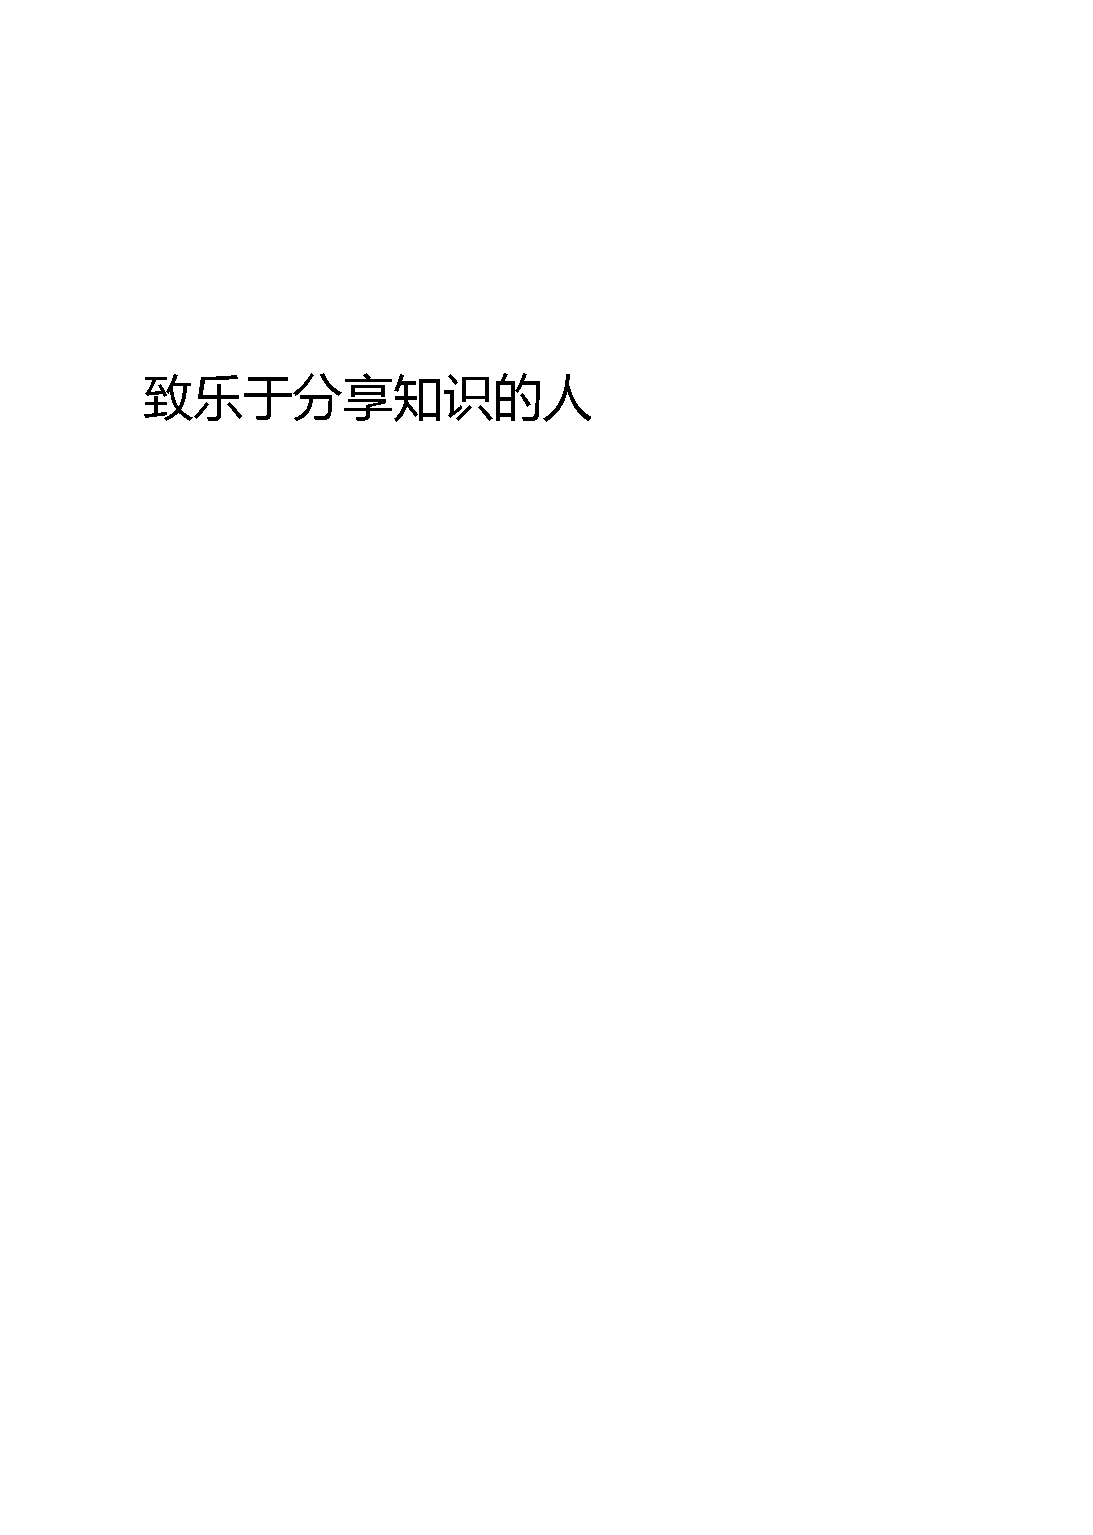
\includepdf{./figures/dedication.pdf}
\end{titlepage}
\frontmatter % 开始罗马数字页码
% 版权声明 关于本书

\chapter*{版权声明}

小时物理百科项目的官方网站为 \href{http://wuli.wiki}{wuli.wiki}, 网站上免费提供本书的网页版和 pdf 版的下载, 仅供\textbf{个人学习使用}. 为了维持项目不断发展, 强烈建议每位读者试读超过 1 小时后在网站上捐款, 我们在此表示衷心感谢. 若未经同意, 请勿以任何方式转载本项目内容(包括插图,代码,网页等). 版权所有, 保留一切权利.

本书不定期更新, 为保证内容质量请及时下载最新版. 当前版本编译于: \today.

\chapter*{小时物理百科}

\subsection{简介}

小时物理百科(以下简称百科)从结构上尝试将教材和百科这两种不同形式的文本融合到一起, 使其既适合初学者自学, 又可按照非常灵活的顺序阅读. 百科计划涵盖物理专业本科课程中的大部分内容, 适用于具有普通高中及以上数学物理水平的读者. 也正因为如此, 百科是一个庞大的工程, 短时间内很难被完成, 所以百科将长期处于更新状态. 为保证阅读质量, 请定期从项目网站下载最新版.

在介绍百科的特点以前,我们先来看一般数理教材的不足:
\begin{enumerate}
\item 需要按顺序学习,不适合初学者快速了解或查找某个话题或知识点. 例如某高中生需要了解角动量的概念, 直接翻开力学书的相关章节发现看不懂, 却又不知道需要先学什么, 也没时间从头先看完高等数学和线性代数的教材再开始学习.
\item 读者不能自己掌握所学内容的深度和严谨性. 例如许多高等数学教材在读者对微积分还没有一个大概的了解时就介绍极限的 $\varepsilon-\delta$ 定义, 微分/积分中值定理, 可微, 可积等. 这些内容对物理的初步学习来说显得过于严谨, 会极大加重学习成本.
\item 不够自洽(self-contained). 一本教材的自洽性指目标读者在学习前是否还需要学习其他教材. 大部分本科物理教材对高中生都是不自洽的, 因为它们往往假设读者具有一定的微积分和线性代数基础.
\end{enumerate}

再来看一般网络百科(如百度百科或维基百科)的不足:
\begin{enumerate}
\item 每个词条都大而全, 涵盖词条标题的所有相关内容.
\item 读者同样不能自己掌握所学内容的深度和严谨程度.
\item 容易出现公式定理的堆积, 缺乏知识点导入和讲述, 缺乏例题, 习题等.
\end{enumerate}

\begin{figure}[ht]
\centering
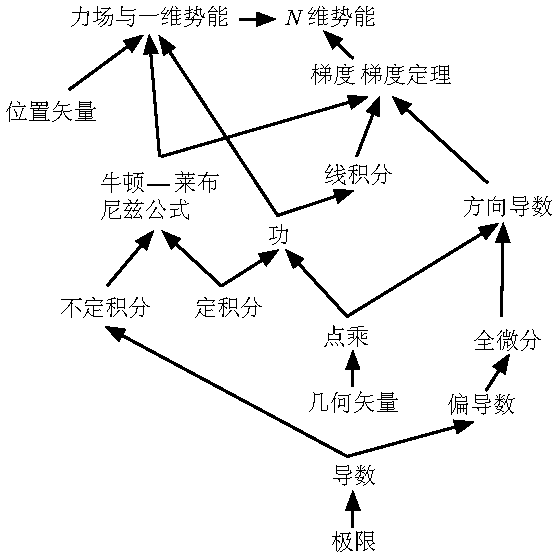
\includegraphics[width=10cm]{./figures/flowchart_example.pdf}
\caption{由“预备知识”画出的知识树(目标词条为“力场\ 势能\upref{V}”)}\label{FrontMatters_fig1}
\end{figure}

为了克服上述困难,百科采用以下形式:
\begin{enumerate}
\item 将知识点划分为词条, 且在每个词条中列出学习该词条前需要先学习哪些词条. 这样相当于建立了一个知识树(如\autoref{FrontMatters_fig1}). 项目网站 \href{http://wuli.wiki}{wuli.wiki} 上可以自动生成任意目标词条的知识树.
\item 采用词条分级,把同一个话题以不同深度,严谨度和适用范围等划分成若干个等级的同名词条.这样读者可以选择螺旋式学习(例如初中,高中,大学物理中所学的话题几乎相同,但程度不同).暂定初级词条从科普开始,尽量少使用数学.随着词条级别升高,会使用适用范围更广的定义,更严谨的表述和更抽象的数学等.
\end{enumerate}

\subsection{词条}
百科内容繁多,不同词条的重要性相去甚远,不建议初学者按照词条的排列顺序依次学习,而是应该以初级词条给出的主线来学习,再根据兴趣和需要阅读其余词条.

理论上来说,读者可以直接跳到最感兴的词条,如果“预备知识”中列出的词条都已经掌握,就可以开始学习该词条,否则就先掌握“预备知识”中的词条.如果“预备知识”出现在词条开始,则必须先掌握,如果出现在正文中,则只有阅读该部分时需要掌握.如果正文中引用了没有出现在“预备知识”中的内容,则读者可自行决定是否阅读.

为了便于书内的跳查,词条之间进行了大量的交叉引用,例如“导数简介\upref{Der}” 右上角中括号中的数字代表被引用词条的页码. 由于每个词条的公式编号都从 1 开始, 引用其他词条中的公式有时会用类似“\autoref{Der_eq2}\upref{Der}” 的格式, 右上角的方括号中是公式所在词条的起始页码. 在本书的 PDF 电子版中,点击该页码即可自动跳转到对应的页面.在电脑上阅读,推荐使用 Adobe Reader 阅读器,在苹果\textsuperscript{\textregistered} 的 iOS 设备上推荐使用 GoodReader 应用( 两个软件都可以在不同的面板中打开同一本书的不同页码). 在 Adobe Reader 中,使用快捷键组合 “Alt +左箭头” 即可返回跳查前的位置,在移动设备的阅读软件中通常也有相应的返回按钮. 由于本书的电子版是原生 PDF(区别于扫描版), 还具有占用设备存储空间小, 便于分享, 便于查找关键字等种种优势.

%\subsection{5.本书符号约定}
%本书尽量使用物理学教科书中最常使用的符号,列出如下
%用粗体表示矢量,如 $\bvec F = m \bvec a$,用非粗体表示标量或矢量的模长,如 $\abs{\bvec F} = F$.同样用粗体表示矩阵,粗体上方加“$\^$”表示算符
% 未完成


% 物理学专业介绍 % 特别强调理科和工科的区别,介绍物理本科物理一般的学习内容
% 只学习最基础的规律,和模型,知识面广,但不复杂
% 由于太基础,会被认为“没有用”,离应用较远.
% 但物理又是其他理工科的基础
% 物理美在哪里? 更像是“艺术”,从几个最基本的假设出发,由数学推导出许多重要的结果.
% 本书遵循的理念:用尽可能少的公理,和尽可能简单的数学推导出结果,但有尽量保持严谨.
% 数学部分不可能做到像高等数学教材一样严谨,只求易懂且满足本书物理部分的使用.
% 均为本科物理专业教科书的标准内容,自己的内容或者超纲内容会在 “超纲内容” 部分中给出
 % 版权声明&关于本书
\setcounter{tocdepth}{1}
\tableofcontents % 生成目录
\mainmatter % 开始阿拉伯数字页码

\part{面向高中生的科普}
\chapter{经典力学}
%------------------------------------------------------------------------------
\entry{经典力学及其他物理理论}{MecThe}
\entry{经典力学}{CM0}
\entry{动量和能量}{CM1}
\entry{角动量}{CM2}

\chapter{电动力学}
%------------------------------------------------------------------------------
\entry{电动力学}{EM0}

\chapter{量子力学}
%------------------------------------------------------------------------------
\entry{量子力学}{QM0}

\chapter{其他}
%------------------------------------------------------------------------------
\entry{天文学常识}{Astro}

\part{数学}
%=======================================
\chapter{数学拾遗}
\entry{二项式定理}{BiNor}
\entry{二项式定理(非整数幂)}{BiNorR}
\entry{三角恒等式}{TriEqv}
\entry{双曲函数}{TrigH}
\entry{充分必要条件}{SufCnd}
\entry{极坐标系}{Polar}
\entry{柱坐标系}{Cylin}
\entry{球坐标系}{Sph}
\entry{球坐标与直角坐标的转换}{SphCar}
\entry{圆锥曲线的极坐标方程}{Cone}
\entry{椭圆的三种定义}{Elips3}
\entry{双曲线的三种定义}{Hypb3}
\entry{抛物线的三种定义}{Para3}
\entry{圆锥曲线的光学性质}{ConOpt}
\entry{复数}{CplxNo}
\entry{复变函数}{Cplx}
\entry{幂函数(复数)}{CPow}
\entry{指数函数(复数)}{CExp}
\entry{三角函数(复数)}{CTrig}

\chapter{一元微积分}
%------------------------------------------------------------------------------
\entry{微积分导航}{Calc}
\entry{极限}{Lim}
\entry{小角正弦极限}{LimArc}
\entry{自然对数底}{E}
\entry{切线与割线}{TanL}
\entry{导数}{Der}
\entry{求导法则}{DerRul}
\entry{反函数求导}{InvDer}
\entry{基本初等函数的导数}{FunDer}
\entry{导数与函数极值}{DerMax}
\entry{用极值点确定函数图像}{DerImg}
\entry{一元函数的微分}{Diff}
\entry{复合函数求导\ 链式法则}{ChainR}
\entry{泰勒展开}{Taylor}
\entry{导数与差分}{DerDif}
\entry{不定积分}{Int}
\entry{换元积分法}{IntCV}
\entry{分部积分法}{IntBP}
\entry{积分表}{ITable}
\entry{定积分}{DefInt}
\entry{牛顿—莱布尼兹公式}{NLeib}
\entry{常微分方程}{ODE}
\entry{一阶线性微分方程}{ODE1}
\entry{二阶常系数齐次微分方程}{Ode2}
\entry{二阶常系数非齐次微分方程}{Ode2N}
\entry{正交函数系}{Fbasis}
\entry{傅里叶级数(三角)}{FSTri}
\entry{傅里叶级数(指数)}{FSExp}
\entry{狄拉克 delta 函数}{Delta}
\entry{傅里叶变换(三角)}{FTTri}
\entry{傅里叶变换(指数)}{FTExp}
\entry{gamma 函数}{Gamma}

\chapter{线性代数 1}
%------------------------------------------------------------------------------
\entry{线性代数导航}{Vector}
\entry{几何矢量}{GVec}
\entry{矢量点乘}{Dot}
\entry{正交归一基底}{OrNrB}
\entry{右手定则}{RHRul}
\entry{矢量叉乘}{Cross}
\entry{矢量叉乘分配律的几何证明}{CrossP}
\entry{连续叉乘的化简}{TriCro}
\entry{高斯消元法解线性方程组}{GAUSS}
\entry{行列式}{Deter}
\entry{三矢量的混合积}{TriVM}
\entry{平面旋转变换}{Rot2DT}
\entry{线性变换}{LTrans}
\entry{矩阵}{Mat}
\entry{逆矩阵}{InvMat}
\entry{平面旋转矩阵}{Rot2D}
\entry{空间旋转矩阵}{Rot3D}
\entry{绕轴旋转矩阵}{RotA}

\chapter{多元微积分与矢量分析}
%------------------------------------------------------------------------------
\entry{偏导数}{ParDer}
\entry{二元函数的极值}{F2Exm}
\entry{最小二乘法}{LstSqr}
\entry{全微分}{TDiff}
\entry{复合函数的偏导\ 链式法则}{PChain}
\entry{全导数}{TotDer}
\entry{矢量的导数\ 求导法则}{DerV}
\entry{一元矢量函数的积分}{IntV}
\entry{方向导数}{DerDir}
\entry{重积分}{IntN}
\entry{极坐标系中单位矢量的偏导}{DPol1}
\entry{正交曲线坐标系}{CurCor}
\entry{曲线坐标系中的重积分}{CrIntN}
\entry{矢量场}{Vfield}
\entry{线积分}{IntL}
\entry{曲面积分\ 通量}{SurInt}
\entry{梯度\ 梯度定理}{Grad}
\entry{散度\ 散度定理}{Divgnc}
\entry{旋度\ 斯托克斯定理}{Curl}
\entry{拉格朗日乘数法}{LagMul}
\entry{一阶线性常微分方程组}{ODEsys}
\entry{多元泰勒展开}{NDtalr}
\entry{雅可比行列式}{JcbDet}
\entry{高斯积分}{GsInt}
\entry{多维球体的体积}{NSphV}

\chapter{线性代数 2}
%-----------------------------------------------------------------------------
\entry{矢量空间}{LSpace}
\entry{代数矢量}{NumVec}
\entry{矩阵与矢量空间}{MatSpc}
\entry{酋矩阵}{UniMat}
\entry{证明闭合曲面的法向量面积分为零}{CSI0}
\entry{超定线性方程组}{OvrDet}
\entry{海森矩阵}{Hesian}
\entry{张量积空间}{DirPro}
\entry{四元数与旋转矩阵}{QuatN}
\entry{CG 系数}{SphCup}
\entry{3j 符号}{ThreeJ}
\entry{6j 符号}{SixJ}
\entry{9j 符号}{NineJ}

\chapter{概率与统计}
%------------------------------------------------------------------------------
% 未完成: 随机变量,概率分布函数
\entry{随机变量的变换}{RandCV}
\entry{高斯分布(正态分布)}{GausPD}
\entry{中心极限定理}{CLT}
\entry{二维随机走动}{RW2D}
\entry{平均值的不确定度}{MeanS}

\chapter{偏微分方程和特殊函数}
%------------------------------------------------------------------------------
\entry{一种 Gibbs 算符的运算方法}{MyNab}
\entry{柱坐标系中的拉普拉斯方程}{CylLap}
\entry{球坐标系中的梯度散度旋度及拉普拉斯算符}{SphNab}
\entry{球坐标系中的拉普拉斯方程}{SphLap}
\entry{球坐标系中的亥姆霍兹方程}{SphHHz}
\entry{勒让德多项式}{Legen}
\entry{连带勒让德多项式}{AsLgdr}
\entry{贝赛尔函数}{Bessel}
\entry{球贝塞尔函数}{SphBsl}
\entry{球谐函数}{SphHar}
\entry{球面波的归一化}{FrNorm}
\entry{平面波的球谐展开}{Pl2Ylm}
\entry{分离变量法与张量积空间}{SVarDP}
\entry{广义球谐函数}{GenYlm}
\entry{误差函数}{Erf}
\entry{虚误差函数}{Erfi}
\entry{超几何函数}{HypGeo}
\entry{库仑函数}{CulmF}

\chapter{其他数学}
\entry{堆放排列组合}{StackC}
\entry{选择的展开定理}{ChExpn}

\part{力学}
%=======================================

\chapter{质点}
%------------------------------------------------------------------------------
\entry{位置矢量\ 位移}{Disp}
\entry{速度\ 加速度(一维)}{VnA1}
\entry{速度\ 加速度}{VnA}
\entry{圆周运动的速度}{CMVD}
\entry{圆周运动的加速度}{CMAD}
\entry{匀加速运动}{ConstA}
\entry{极坐标中的速度和加速度}{PolA}
\entry{牛顿运动定律\ 惯性系}{New3}
\entry{功\ 功率}{Fwork}
\entry{动能\ 动能定理(单个质点)}{KELaw1}
\entry{力场\ 势能}{V}
\entry{机械能守恒(单个质点)}{ECnst}
\entry{动量\ 动量定理(单个质点)}{PLaw1}
\entry{角动量\ 角动量定理\ 角动量守恒(单个质点)}{AMLaw1}
\entry{简谐振子}{SHO}
\entry{受阻落体}{RFall}
\entry{单摆}{Pend}
\entry{傅科摆}{Fouclt}
\entry{惯性力}{Iner}
\entry{离心力}{Centri}
\entry{科里奥利力}{Corio}
\entry{地球表面的科里奥利力}{ErthCf}

\chapter{质点系与刚体}
%------------------------------------------------------------------------------
\entry{常见物理量}{PhyQty}
\entry{物理学常数定义}{Consts}
\entry{自由度}{DoF}
\entry{质点系}{PSys}
\entry{质心\ 质心系}{CM}
\entry{刚体}{RigBd}
\entry{质点系的动量}{SysP}
\entry{动量定理\ 动量守恒}{PLaw}
\entry{质点系的动能\ 柯尼西定理}{Konig}
\entry{力矩}{Torque}
\entry{刚体的静力平衡}{RBSt}
\entry{角动量}{AngMom}
\entry{角动量定理\ 角动量守恒}{AMLaw}
\entry{二体系统}{TwoBD}
\entry{二体碰撞}{TwoCld}
\entry{刚体的绕轴转动\ 转动惯量}{RigRot}
\entry{平行轴定理与垂直轴定理}{MIthm}
\entry{常见几何体的转动惯量}{ExMI}
\entry{刚体的平面运动方程}{RBEM}
\entry{浮力}{Buoy}

\chapter{振动与波动}
%------------------------------------------------------------------------------
\entry{振动的指数形式}{VbExp}
\entry{受阻简谐振子}{SHOf}
\entry{简谐振子受迫运动}{SHOfF}
\entry{平面波}{PWave}
\entry{一维波动方程}{WEq1D}
% 未完成 边界条件 (两条密度不同的绳子)

\chapter{中心力场问题}
\entry{万有引力\ 引力势能}{Gravty}
\entry{无量纲的物理公式}{NoUnit}
\entry{球体的引力场}{SphF}
\entry{中心力场问题}{CenFrc}
\entry{开普勒问题}{CelBd}
\entry{开普勒三定律}{Keple}
\entry{拉普拉斯—龙格—楞次矢量}{LRLvec}
\entry{轨道方程\ 比耐公式}{Binet}
\entry{开普勒第一定律的证明}{Keple1}
\entry{开普勒第二和第三定律的证明}{Keple2}
\entry{反开普勒问题}{InvKep}
% 散射, 定义微分截面 % d sigma/d Omega 真的就是面积元比对应的立体角元
\entry{散射}{Scater}\newpage
\entry{卢瑟福散射}{RuthSc}

\chapter{理论力学}
%------------------------------------------------------------------------------
\entry{拉格朗日方程}{Lagrng}
\entry{达朗贝尔定理}{dAlbt}
\entry{哈密顿原理}{HamPrn}
\entry{哈密顿正则方程}{HamCan}
\entry{闭合轨道的条件}{ClsOrb}
\entry{经典力学笔记}{ClsMec}
\entry{转动惯量张量}{ITensr}

\chapter{轨道力学}
%------------------------------------------------------------------------------
\entry{轨道参数 时间变量}{OribP}
\entry{限制性三体问题}{TriLim}
\entry{雅可比常量}{JConst}
\entry{拉格朗日点}{LPoint}

\part{电动力学}
%=======================================
\chapter{电动力学 1}
%------------------------------------------------------------------------------
\entry{电流}{I}
\entry{电荷守恒\ 电流连续性方程}{ChgCsv}
\entry{电势\ 电势能}{QEng}
\entry{导体}{Cndctr}
\entry{电容}{Cpctor}
\entry{电场的高斯定理}{EGauss}
\entry{电场的能量}{EEng}
\entry{LC 振荡电路}{LC}
\entry{比奥萨伐尔定律}{BioSav}
\entry{安培环路定理}{AmpLaw}
\entry{洛伦兹力}{Lorenz}
\entry{磁场的能量}{BEng}
\entry{磁通量}{BFlux}
\entry{安培力}{FAmp}
\entry{磁场中闭合电流的合力}{EBLoop}
\entry{磁场中闭合电流的力矩}{EBTorq}
\entry{法拉第电磁感应定律}{FaraEB}

\chapter{电动力学 2}
%------------------------------------------------------------------------------
\entry{电磁场标势和矢势}{EMPot}
\entry{规范变换}{Gauge}
\entry{电磁场的能量守恒\ 坡印廷矢量}{EBS}
\entry{麦克斯韦方程组}{MWEq}
\entry{麦克斯韦方程组(介质)}{MWEq1}
\entry{非齐次亥姆霍兹方程\ 推迟势}{RetPot}
\entry{电场波动方程}{EWEq}
\entry{真空中的平面电磁波}{VcPlWv}
\entry{介质中的波动方程}{MedWF}
\entry{菲涅尔公式}{Fresnl}
\entry{盒中的电磁波}{EBBox}
\entry{电磁场的动量守恒\ 动量流密度张量}{EBP}
\entry{磁旋比\ 玻尔磁子}{BohMag}

\chapter{电动力学 3}
%------------------------------------------------------------------------------
\entry{拉格朗日电磁势}{EMLagP}
\entry{电磁场角动量分解}{EMAMSp}

\part{量子力学}
%=======================================
% 考虑一下选取什么样的讲解顺序? 大概就是先介绍线性代数(包括离散和连续的矢量空间,狄拉克符号),介绍量子力学的基本公设(本征方程,算符,时间演化三步法),德布罗意波,然后推导平均值公式,位置动量表象的变换,束缚态,散射,等等

% 未完成 讲讲为什么定态波函数一定是实数函数? 实数波函数为什么会有动量平均值为零?
% 未完成 x,p不确定原理,一般的不确定原理, 高斯波包时取等号.
% 未完成 束缚态的一般性质: 节点数, 对称性 (偶势能的基态是偶函数), 简并性(一维情况不简并)

\chapter{量子力学 1}
%------------------------------------------------------------------------------
\entry{玻尔原子模型}{BohrMd}
\entry{原子单位}{AU}
\entry{量子力学的基本假设}{QM1}
\entry{高斯波包}{GausWP}
\entry{无限深势阱}{ISW}
\entry{升降算符}{RLop}
\entry{简谐振子(升降算符)}{QSHOop}
\entry{简谐振子升降算符归一化}{QSHOnr}
\entry{简谐振子(级数)}{QSHOxn}
\entry{有限深球势阱}{FiSph}
\entry{算符对易与共同本征函数}{Commut}
\entry{类氢原子的约化质量}{HRMass}
\entry{概率流密度}{PrbJ}
\entry{算符的矩阵表示}{OpMat}
\entry{轨道角动量}{QOrbAM}
\entry{轨道角动量升降算符归一化}{QLNorm}
\entry{自旋角动量}{Spin}

\chapter{量子力学 2}
%------------------------------------------------------------------------------
\entry{算符的指数函数\ 波函数传播子}{OpExp}
\entry{平移算符}{tranOp}
\entry{旋转算符}{rotOp}
\entry{角动量加法}{AMAdd}
\entry{能量归一化}{EngNor}
\entry{氢原子基态的波函数}{HWF0}
\entry{球坐标和柱坐标中的定态薛定谔方程}{RadSE}
\entry{球坐标中的薛定谔方程}{RYTDSE}
\entry{量子力学中的变分法}{QMVar}
\entry{数值解一维薛定谔方程(试射法)}{NSES}
\entry{含时微扰理论}{TDPT}
\entry{几种含时微扰}{TDPEx}
\entry{含连续态的微扰理论}{PTCont}
\entry{量子散射\ 分波展开}{ParWav}
\entry{波恩近似(散射)}{BornSc}
\entry{质心系中的多粒子问题}{SECM}
\entry{三维简谐振子(球坐标)}{SHOSph}
\entry{球面散射态与平面散射态的转换}{Scatt2}
\entry{库仑波函数}{CulmWf}
\entry{量子力学的基本假设}{QMPos}
\entry{带电粒子的薛定谔方程}{EMTDSE}
\entry{电磁场中的单粒子薛定谔方程}{QMEM}
\entry{电磁场中的类氢原子}{EMHydr}
\entry{Volkov 波函数}{Volkov}
\entry{氢原子的选择定则}{SelRul}
\entry{康普顿散射}{Comptn}

\chapter{量子力学与量子场论}
%------------------------------------------------------------------------------
\entry{本章导航}{QFIntro}
\entry{基本概念}{Basics}
\entry{全同粒子的统计}{IdParS}
\entry{近似理论:微扰}{AprPtr}
\entry{角动量}{QMAM}
% 第六章直接从 sakurai 翻译, 后面的一些内容非常零碎跳过
\entry{冷原子基本知识}{UCBas}
\entry{两个原子间的相互作用}{TwoAtF}
\entry{Feshbach 共振}{FeshRs}
\entry{BCS-BEC Crossover 的平均场描述}{BCSBEC}
\entry{BEC 超流}{BECSup}
\bibentry{laserdog}

\part{原子分子物理}
%=======================================
\entry{氢原子的波函数}{HWF}
\entry{电子轨道与元素周期表}{Ptable}
%------------------------------------------------------------------------------

\part{统计力学}
%=======================================
\entry{理想气体状态方程}{PVnRT}
\entry{分子平均碰壁数}{AvgHit}
\entry{统计力学公式大全}{StatEq}
\entry{相空间}{PhSpace}
\entry{理想气体的状态密度(相空间)}{IdSDp}
\entry{理想气体单粒子能级密度}{IdED1}
\entry{理想气体(微正则系综法)}{IdNCE}
\entry{正则系宗法}{CEsb}
\entry{理想气体(正则系宗法)}{IdCE}
\entry{理想气体(巨正则系综法)}{IdMCE}
\entry{等间隔能级系统(正则系宗)}{EqCE}
\entry{巨正则系综法}{MCEsb}
\entry{量子气体(单能级巨正则系综法)}{QGs1ME}
\entry{量子气体(巨正则系宗)}{QGsME}

\part{计算物理}
%=======================================
\chapter{Matlab 及其他工具}
% 未完成 Mathematica
% 未完成 Wolfram Alpha
%------------------------------------------------------------------------------
\entry{计算物理导航}{NumPhy}
\entry{Matlab 简介}{Matlab}
\entry{Matlab 的变量与矩阵}{MatVar}
\entry{Matlab 的判断与循环}{MIfFor}
\entry{Matlab 的函数}{MatFun}
\entry{Matlab 画图}{MatPlt}
\entry{Matlab 的程序调试及其他功能}{MatOtr}

\chapter{数值验证及常用算法}
%------------------------------------------------------------------------------
\entry{二项式定理(非整数幂)的数值验证}{BiNorM}
\entry{二分法}{Bisec}
\entry{多区间二分法}{MBisec}
\entry{冒泡法}{Bubble}
\entry{高斯消元法程序}{GauEli}
\entry{Nelder-Mead 算法}{NelMea}
\entry{最小二乘法的数值计算}{CurFit}
\entry{数值积分(梯形法)}{NumInt}
\entry{稀疏矩阵}{SprMat}
\entry{函数求值}{SpcFun}
\entry{离散傅里叶变换}{DFT}
\entry{离散正弦变换}{DST}

\chapter{微分方程数值解}
%------------------------------------------------------------------------------
\entry{简谐振子受迫运动的简单数值计算}{SHOFN}
\entry{天体运动的简单数值计算}{KPNum0}
\entry{常微分方程(组)的数值解}{OdeNum}
\entry{中点法解常微分方程(组)}{OdeMid}
\entry{四阶龙格库塔法}{OdeRK4}

\chapter{一维薛定谔方程数值解}
%-------------------------------------------------------------------------------
\entry{一维势能束缚态数值解(试射法)}{BndSho}

\chapter{氢原子薛定谔方程数值解}
%-------------------------------------------------------------------------------
\entry{Crank-Nicolson 算法(一维)}{CraNic}
\entry{Hartree-Fork 方法}{HarFor}
\entry{Gauss-Lobatto 积分}{GLquad}
\entry{FEDVR 算法}{FEDVR}
\entry{Lanczos 算法}{Lanc}
\entry{虚时间法求基态波函数}{ImgT}
\entry{氢原子球坐标数值解 TDSE}{HTDSE}

\chapter{氦原子薛定谔方程数值解}
%-------------------------------------------------------------------------------
\entry{氦原子数值解 TDSE}{HeTDSE}

\part{小时物理笔记}
%=======================================
% 不要在这里修改,在 PhysWikiNote.tex 中修改后再复制过来
\chapter{SFA}
%-------------------------------------------------------------------------------
\entry{FROG}{Frog}
\entry{Frog-Crab}{FrogCr}

\chapter{AMO2}
%-------------------------------------------------------------------------------
\entry{多通道散射}{MulSct}
\entry{Adiabatic 笔记}{Adibat}

\chapter{杂}
%-------------------------------------------------------------------------------
\entry{晶体衍射}{CrysDf}
\end{document}
